\section{Forsøgsplan}

For at validere testresultaterne vil vi benytte os af joint histograms. For hvert sCT vi generer har vi det korrekte CT. Ved at plotte sCT værdier som x koordinaten og CT værdier som y koordinaten får vi en visuel repræsentation af ligheden mellem billederne. Hvis resultatet er identisk vil der optræde en enkelt lige linje fra (0,0) til (max,max). Jo mere forskellige de er jo længere fra den lige linje ligger punkterne.

Fordelen ved denne metode er at vi nemt kan aflæse hvilke værdier vi har de største problemer med. Hvis vi har meget stor afvigelse i knoglerne vil vi få en stor klump omkring nul, mens der kan være store ligheder i det bløde væv der så giver en pæn linje omkring minus 500.

Derudover er det samme valideringsmetode der bruges af Johannson et al., og vi vil derfor kunne sammenligne vores værdier med deres.

For at finde ud af om vores sCT er godt nok til attenuationskorrektion af PET billeder vil vi generere PET billeder med vores sCT og det rigtige CT. Vi kan herefter konstruere et nyt billede, der er baseret på den procentvise forskel imellem PET/CT og PET/sCT. 

Ud fra procentsforskelsbilledet kan vi se hvilke regioner der er forskellige fra PET/CT billedet, og giver samtidigt et godt overblik over hvor godt vores PET/sCT billede er blevet.

Begge disse valideringsmetoder er objektive men skal evalueres manuelt. Vi har ikke en metode til at give et enkelt tal for hvor godt vores PET/sCT billede er blevet. Vi forventer også at kvaliteten af sCT billedet, og dermed også PET/sCT billedet vil variere meget.


Da flere af FullCT billederne er lavet uden en perfekt maske, som skjuler hovedholder og nakkestøtten på CT billedet, har vi valgt at generere nye FullCT baseret på CT billeder påført vores maske. Da støj rundt omkring hovedet påvirker attenuation korrektionen fik vi billeder med meget stor afvigelse imod den bagerste del af kraniet. Da vi er sikre på at både sCT og CT billederne er påført samme maske, er der større sandsynlighed for at vi sammenligner vores algoritme frem for støj. Der kan dog stadig fremkomme små rester af hovedstøtten tæt på kraniet, men det ser ikke ud til at være et problem.

\todo{tekst, beskriv joint histogram, omdoeb faldgrupper}

\subsection{Leave-one-out cross validation (LOOCV)}
\subsubsection{Fremgangsmåde}
Leave-one-out cross validation (LOOCV) er en gængs metode der bruges til at teste korrektheden af en algoritme. I alt sin enkelthed går metoden ud på at vi udvælger fem patienter. Fra de fem patienter lægger vi en patient til side, fx. den første patient, og træner algoritmen på de resterende fire patienter. Derefter udregner vi et sCT for den første patient. Vi gør herefter det samme igen, men udelader patient nummer to, træner på de resterende fire og udregner nummer to's sCT. 

Ved at rotere træningssættet får vi testet metoden med data fra forskellige patienter, og vi får en basis for at sammenligne sCT'et.

Vi har valgt dette test scenarie for at kunne sammenligne vores resultater med Johansson et al, da de benytter samme test.

\subsubsection{Forventning}
Vi forventer at vores joint histograms bliver dårligere end Johannsons's, da vores hidtidige sCT er visuelt dårligere end deres.


\subsubsection{Faldgrupper}
For at opnå stabile resultater er vi nødt til at filtrere patienter med artifakter fra. Da artifakter repræsentere områder med manglende data, tror vi det er nødvendigt for kvaliteten af vores algoritme, at de bliver sorteret fra.

\subsubsection{Resultat}

Eftersom det primære mål med denne test er at sammeligne os med Johannsonn et al. har vi valgt at genskabe de samme figure.

\begin{figure}
    \centering
    \begin{subfigure}[b]{0.45\textwidth}
        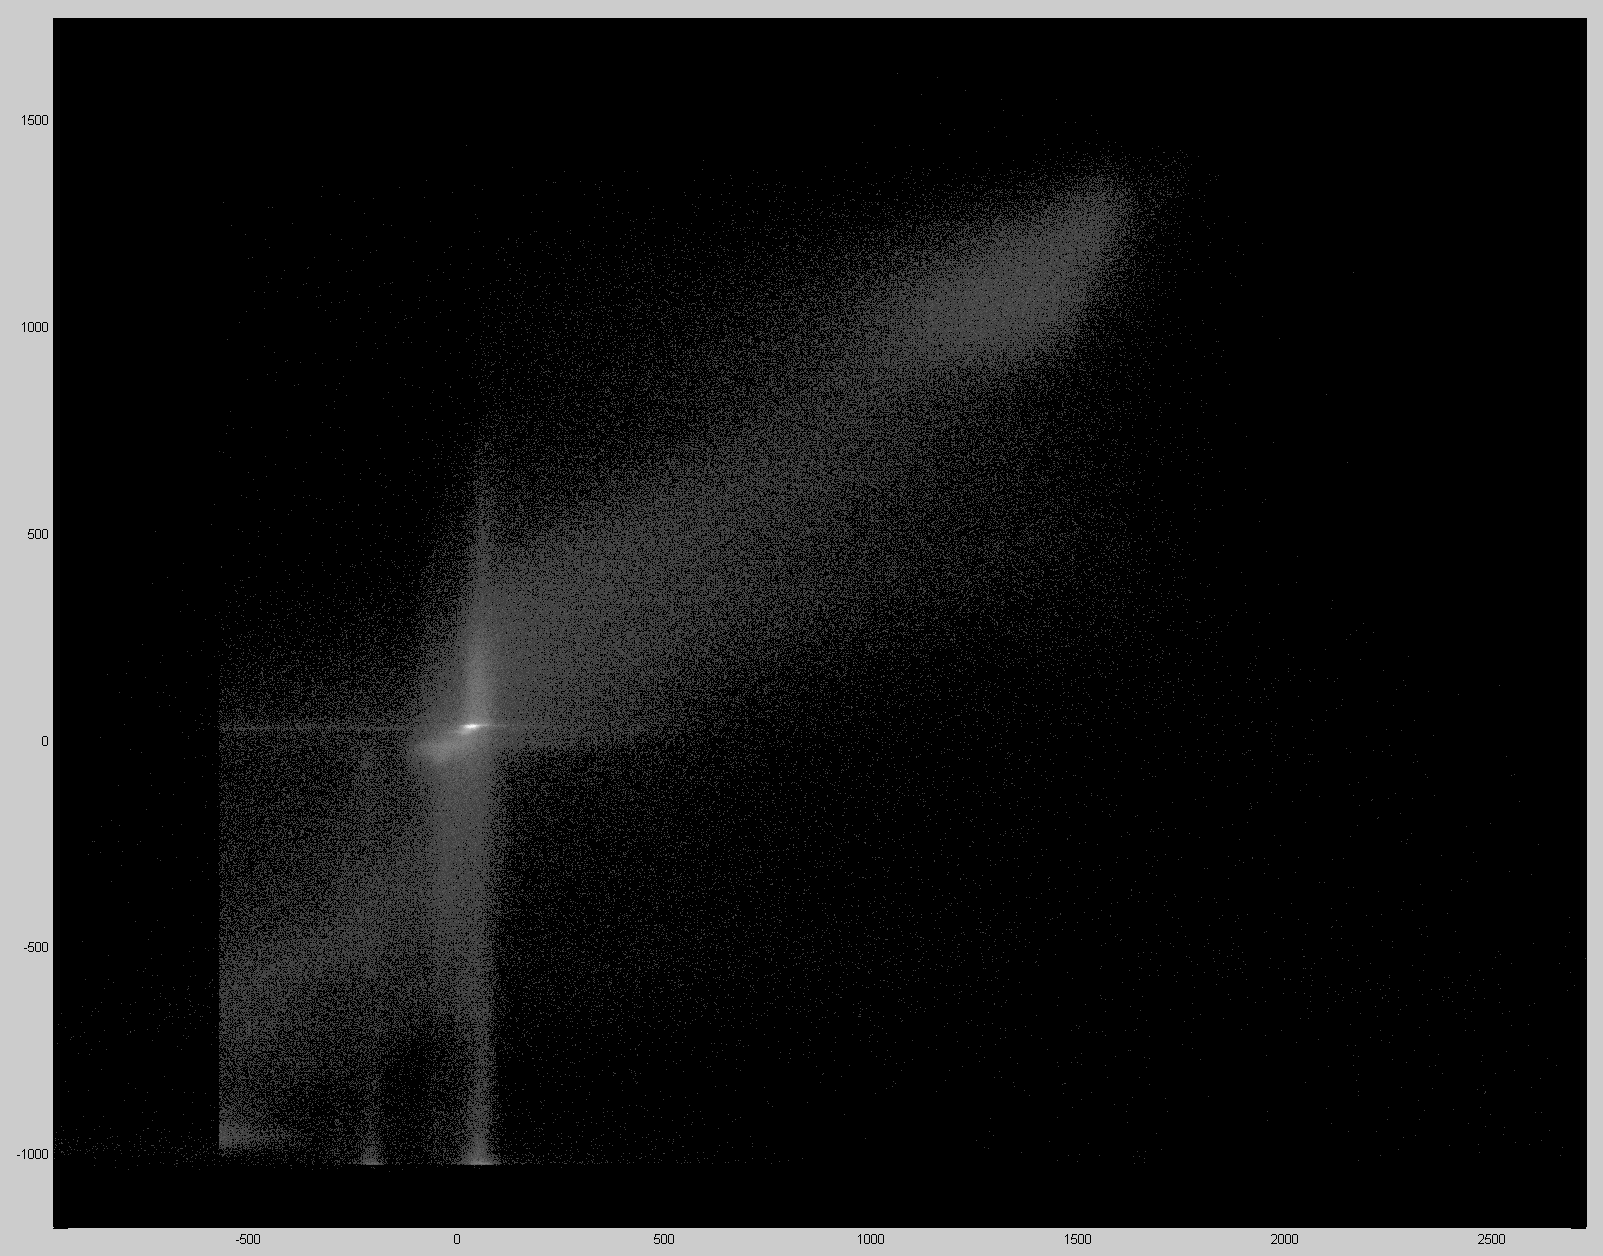
\includegraphics[width=0.75\textwidth]{loocv_joint_histogram.png}
        \caption{Fælleshistogram for patient 1.}
        \label{fig:loocv_j_h}
    \end{subfigure}\hfill
    \begin{subfigure}[b]{0.45\textwidth}
        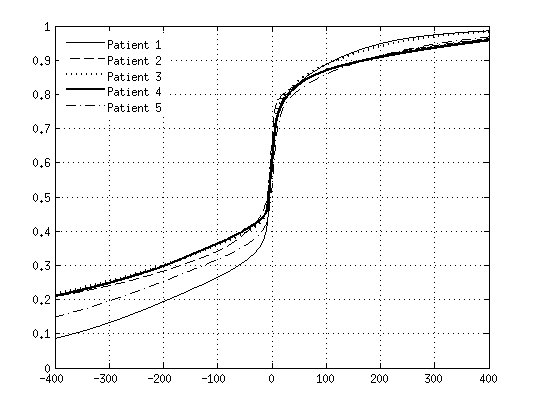
\includegraphics[width=0.75\textwidth]{cumm_diff_loocv.png}
        \caption{kommulativt diagram for alle patienter i LOOCV forsøget.}
        \label{fig:cumm_diff_loocv}
    \end{subfigure}
    \caption{På figur~\ref{fig:loocv_j_h} ses et fælleshistogram for patient 1. CT værdier ud af x-aksen og sCT værdier ud af y aksen. På figur~\ref{fig:loocv_j_h} ses den kommulative afvigelse af sCT fra CT normaliseret til 1.}
    \label{fig:loocv}
\end{figure}

På fælleshistogrammet på figur~\ref{fig:loocv_j_h} kan vi se to koncentrationer af punkter lige omkring 0 HU. Under nul kommer vi ud i luft og blødt væv. Over 0 kan vi se hvordan knoglen ligger. Omkring 500 findes den største spredning af punkterne.

På det kommulative diagram på figur~\ref{fig:cumm_diff_loocv} kan vi se at vi generelt har et problem med for lave værdier i sCT i forhold til CT. Mere end 40\% af punkterne ligger for lavt.

Ud fra procent difference (PD) billederne kan vi se at algoritmen levere nogenlunde stabile resultater. Men vi kan også se at der er store problemer ved ventriklerne, hvor den procentvise forskel på flere af billederne sniger sig op over de ti procent.

Hvis vi ser på et PD billede lagt over et MR billede er det tydeligt at jo tættere på hjerneskallen vi kommer, jo større bliver afvigelsen.

Det er ikke muligt for os at evaluere korrektheden af algoritmen omkring mund og næse regionen da langt de fleste T2 sekvenser ikke indeholder data så langt nede. Ligeså er der problemer i toppen af kraniet da T2 sekvenserne også mangler en skive eller to, og derfor ikke har hele hjerneskallen med.

I gennemsnit er der lidt under ti procent afvigelse i selve hjernen.

\begin{figure}
    \centering
    \begin{subfigure}[b]{0.3\textwidth}
        \caption{CT for patient 1.}
        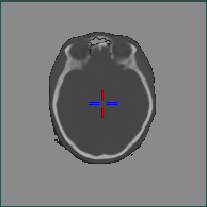
\includegraphics[width=0.75\textwidth]{colager/loocv_ct/loocv_010476_ct.png}
        \label{col:loocv_ct_pat1_ct}
    \end{subfigure}\hfill
    \begin{subfigure}[b]{0.3\textwidth}
        \caption{sCT.}
        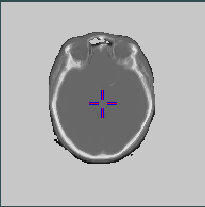
\includegraphics[width=0.75\textwidth]{colager/loocv_ct/loocv_010476_sct.png}
        \label{col:loocv_ct_pat1_sct}
    \end{subfigure}\hfill
    \begin{subfigure}[b]{0.3\textwidth}
        \caption{Differens.}
        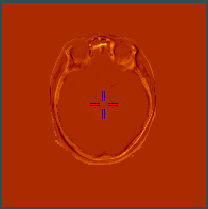
\includegraphics[width=0.75\textwidth]{colager/loocv_ct/loocv_010476_sub.png}
        \label{col:loocv_ct_pat1_sub}
    \end{subfigure}\\
    \begin{subfigure}[b]{0.3\textwidth}
        \caption{CT for patient 2.}
        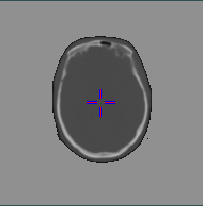
\includegraphics[width=0.75\textwidth]{colager/loocv_ct/loocv_010769_ct.png}
        \label{col:loocv_ct_pat2_ct}
    \end{subfigure}\hfill
    \begin{subfigure}[b]{0.3\textwidth}
        \caption{sCT.}
        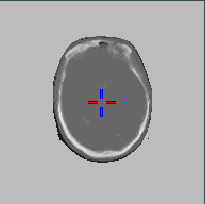
\includegraphics[width=0.75\textwidth]{colager/loocv_ct/loocv_010769_sct.png}
        \label{col:loocv_ct_pat2_sct}
    \end{subfigure}\hfill
    \begin{subfigure}[b]{0.3\textwidth}
        \caption{Differens.}
        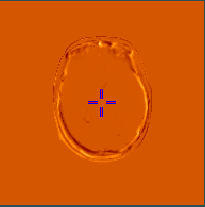
\includegraphics[width=0.75\textwidth]{colager/loocv_ct/loocv_010769_sub.png}
        \label{col:loocv_ct_pat2_sub}
    \end{subfigure}\\
    \begin{subfigure}[b]{0.3\textwidth}
        \caption{CT for patient 3.}
        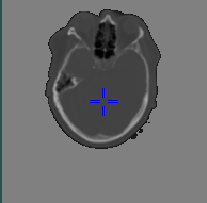
\includegraphics[width=0.75\textwidth]{colager/loocv_ct/loocv_010850_ct.png}
        \label{col:loocv_ct_pat3_ct}
    \end{subfigure}\hfill
    \begin{subfigure}[b]{0.3\textwidth}
        \caption{sCT.}
        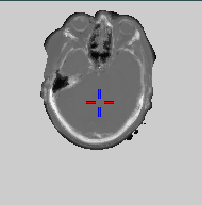
\includegraphics[width=0.75\textwidth]{colager/loocv_ct/loocv_010850_sct.png}
        \label{col:loocv_ct_pat3_sct}
    \end{subfigure}\hfill
    \begin{subfigure}[b]{0.3\textwidth}
        \caption{Differens.}
        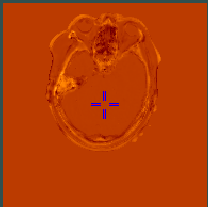
\includegraphics[width=0.75\textwidth]{colager/loocv_ct/loocv_010850_sub.png}
        \label{col:loocv_ct_pat3_sub}
    \end{subfigure}\\
    \begin{subfigure}[b]{0.3\textwidth}
        \caption{CT for patient 4.}
        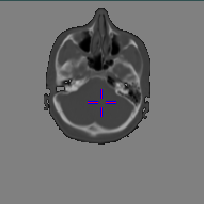
\includegraphics[width=0.75\textwidth]{colager/loocv_ct/loocv_010960_ct.png}
        \label{col:loocv_ct_pat4_ct}
    \end{subfigure}\hfill
    \begin{subfigure}[b]{0.3\textwidth}
        \caption{sCT.}
        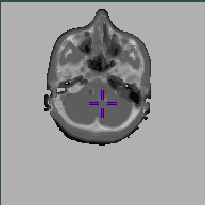
\includegraphics[width=0.75\textwidth]{colager/loocv_ct/loocv_010960_sct.png}
        \label{col:loocv_ct_pat4_sct}
    \end{subfigure}\hfill
    \begin{subfigure}[b]{0.3\textwidth}
        \caption{Differens.}
        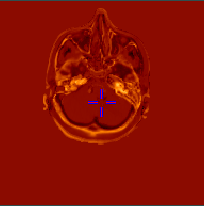
\includegraphics[width=0.75\textwidth]{colager/loocv_ct/loocv_010960_sub.png}
        \label{col:loocv_ct_pat4_sub}
    \end{subfigure}\\
    \begin{subfigure}[b]{0.3\textwidth}
        \caption{CT for patient 5.}
        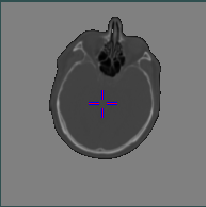
\includegraphics[width=0.75\textwidth]{colager/loocv_ct/loocv_011030_ct.png}
        \label{col:loocv_ct_pat5_ct}
    \end{subfigure}\hfill
    \begin{subfigure}[b]{0.3\textwidth}
        \caption{sCT.}
        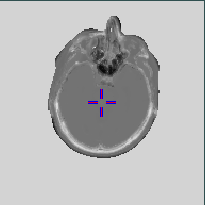
\includegraphics[width=0.75\textwidth]{colager/loocv_ct/loocv_011030_sct.png}
        \label{col:loocv_ct_pat5_sct}
    \end{subfigure}\hfill
    \begin{subfigure}[b]{0.3\textwidth}
        \caption{Differens.}
        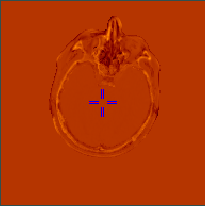
\includegraphics[width=0.75\textwidth]{colager/loocv_ct/loocv_011030_sub.png}
        \label{col:loocv_ct_pat5_sub}
    \end{subfigure}
    \caption{CT, sCT og differencen imellem dem for de fem patienter.}
    \label{col:loocv_ct}
\end{figure}

\begin{figure}
    \centering
    \begin{subfigure}[b]{0.3\textwidth}
        \caption{FullCT for patient 1.}
        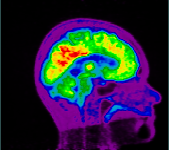
\includegraphics[width=0.75\textwidth]{colager/loocv_pet/loocv_010476_pet_ct.png}
        \label{col:loocv_pet_pat1_ct}
    \end{subfigure}\hfill
    \begin{subfigure}[b]{0.3\textwidth}
        \caption{PET baseret på sCT.}
        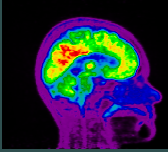
\includegraphics[width=0.75\textwidth]{colager/loocv_pet/loocv_010476_pet_sct.png}
        \label{col:loocv_pet_pat1_sct}
    \end{subfigure}\hfill
    \begin{subfigure}[b]{0.3\textwidth}
        \caption{Procentdifferens.}
        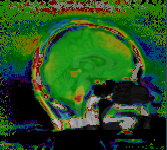
\includegraphics[width=0.75\textwidth]{colager/loocv_pet/loocv_010476_pet_pd.png}
        \label{col:loocv_pet_pat1_pd}
    \end{subfigure}\\
    \begin{subfigure}[b]{0.3\textwidth}
        \caption{FullCT for patient 2.}
        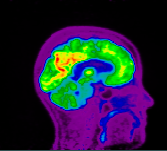
\includegraphics[width=0.75\textwidth]{colager/loocv_pet/loocv_010769_pet_ct.png}
        \label{col:loocv_pet_pat2_ct}
    \end{subfigure}\hfill
    \begin{subfigure}[b]{0.3\textwidth}
        \caption{PET baseret på sCT.}
        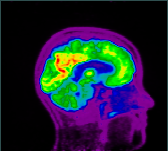
\includegraphics[width=0.75\textwidth]{colager/loocv_pet/loocv_010769_pet_sct.png}
        \label{col:loocv_pet_pat2_sct}
    \end{subfigure}\hfill
    \begin{subfigure}[b]{0.3\textwidth}
        \caption{Procentdifferens.}
        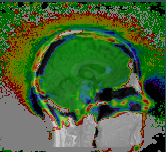
\includegraphics[width=0.75\textwidth]{colager/loocv_pet/loocv_010769_pet_pd.png}
        \label{col:loocv_pet_pat2_sub}
    \end{subfigure}\\
    \begin{subfigure}[b]{0.3\textwidth}
        \caption{FullCT for patient 3.}
        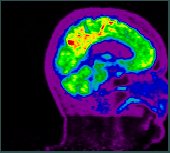
\includegraphics[width=0.75\textwidth]{colager/loocv_pet/loocv_010850_pet_ct.png}
        \label{col:loocv_pet_pat3_ct}
    \end{subfigure}\hfill
    \begin{subfigure}[b]{0.3\textwidth}
        \caption{PET baseret på sCT.}
        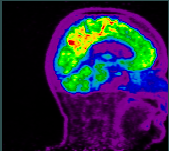
\includegraphics[width=0.75\textwidth]{colager/loocv_pet/loocv_010850_pet_sct.png}
        \label{col:loocv_pet_pat3_sct}
    \end{subfigure}\hfill
    \begin{subfigure}[b]{0.3\textwidth}
        \caption{Procentdifferens.}
        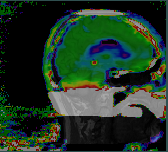
\includegraphics[width=0.75\textwidth]{colager/loocv_pet/loocv_010850_pet_pd.png}
        \label{col:loocv_pet_pat3_pd}
    \end{subfigure}\\
    \begin{subfigure}[b]{0.3\textwidth}
        \caption{FullCT for patient 4.}
        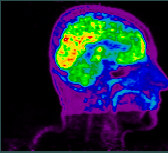
\includegraphics[width=0.75\textwidth]{colager/loocv_pet/loocv_010960_pet_ct.png}
        \label{col:loocv_pet_pat4_ct}
    \end{subfigure}\hfill
    \begin{subfigure}[b]{0.3\textwidth}
        \caption{PET baseret på sCT.}
        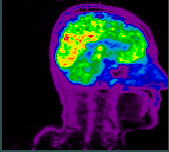
\includegraphics[width=0.75\textwidth]{colager/loocv_pet/loocv_010960_pet_sct.png}
        \label{col:loocv_pet_pat4_sct}
    \end{subfigure}\hfill
    \begin{subfigure}[b]{0.3\textwidth}
        \caption{Procentdifferens.}
        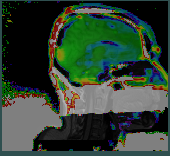
\includegraphics[width=0.75\textwidth]{colager/loocv_pet/loocv_010960_pet_pd.png}
        \label{col:loocv_pet_pat4_pd}
    \end{subfigure}\\
    \begin{subfigure}[b]{0.3\textwidth}
        \caption{FullCT for patient 5.}
        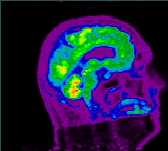
\includegraphics[width=0.75\textwidth]{colager/loocv_pet/loocv_011030_pet_ct.png}
        \label{col:loocv_pet_pat5_ct}
    \end{subfigure}\hfill
    \begin{subfigure}[b]{0.3\textwidth}
        \caption{PET baseret på sCT.}
        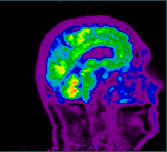
\includegraphics[width=0.75\textwidth]{colager/loocv_pet/loocv_011030_pet_sct.png}
        \label{col:loocv_pet_pat5_sct}
    \end{subfigure}\hfill
    \begin{subfigure}[b]{0.3\textwidth}
        \caption{Procentdifferens.}
        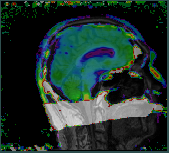
\includegraphics[width=0.75\textwidth]{colager/loocv_pet/loocv_011030_pet_pd.png}
        \label{col:loocv_pet_pat5_pd}
    \end{subfigure}
    \caption{CT, sCT og procentdifferencen for de fem patienter. Farveskalaen for procentdifferencen går fra -20 til 20.}
    \label{col:loocv_pet}
\end{figure}

\subsection{Over tid}
\subsubsection{Fremgangsmåde}

Der har fra Rigshopitalets side været en interesse i at undersøge, om
metoden ville virke fremadrettet. Altså om en model trænet på noget data
fra en periode, ville kunne bruges til at udregne et sCT for en patient
fra en helt anden periode. 

For at undersøge dette, har vi taget de seks
tidligst optagede patienter med UTE, som ikke havde artifakter, og
var nye nok til at den T2 serie, som vi træner udfra, er optaget.
Derudover tog vi de seks nyeste UTE patienter, ligeledes uden artikater.

\todo{Datoer}

Derefter trænede vi to modeller. En på de gamle patienter, og en på de
nye. Vi lavede da sCT'er for de gamle patienter, på den nye model og
omvendt. For at vurdere om det virker, vil vi benytte samme fremgangsmåde,
som i LOOCV, og hvis resultaterne minder tilstrækkeligt, om dem fra det
tidligere forsøg, vil det være godt nok. Hvis forsøget ikke giver gode
resultater vi ldet betyde, at man løbende skal træne nye modeller, for at
få gode resultater.

\subsubsection{Forventning}

Forventningen er sCT af samme kvalitet, som dem ved LOOCV-forsøget.
Ændringer på PET/MR scanneren kan sagtens påvirke resultaterne af et MR
scan, men så længe ændringerne er nogenlunde lige fordelt, så er det ikke
et problem, da MR-units er arbitrære og ikke kan sammenlignes fra scan til
scan. Der skal være er en region af hjernen, som bliver målt anderledes i
forhold til resten af hjernen før der bliver problemer.

\subsubsection{Faldgrupper}

Vores scanninger foreløber ikke over så lang en periode, og vi har
kun valgt at sammenligne to perioder. Så kan det for det første
bare ikke have haft nogen effekt med de hidtidige ændringer eller
måske har der været flere ændringer indimellem, som har påvirket
scanningsresultaterne, men på seneste tidspunkt er resultaterne meget
lig de tidlige.